\pagestyle{fancy}
\setlength{\headheight}{16pt}
\fancyhead{} % clear all header fields
\fancyhead[L]{\textbf{TAM 514 Homework 5}}
\fancyhead[C]{Songyuan Cui}
\fancyhead[R]{\textbf{Spring 2025}}
\fancyfoot{} % clear all footer fields
\fancyfoot[C]{\thepage}

\begin{problem}
    \textbf{1 (100 pts).} 
    Compute the Green's function for the eigenvalue problem of the simply supported Euler-Bernoulli beam:
    \begin{equation}
    \begin{gathered}
        u''''(x) - \lambda u(x) = f(x), ~~~~ 0 \leq x \leq 1 \\
        u(0) = u''(0) = u(1) = u''(1) = 0
    \end{gathered}
    \end{equation}
    You should use two alternative definitions for the linear operator and construct two different Green's function formulations. 
    In each case verify that the Green's function is symmetric with respect to its arguments. 
    Then, use the derived Green's functions to convert the boundary value problem to an integral equation (do that for each of the two Green's functions). 
    Hint: In the first case define $L[u] = u''''(x)$ and in the second $L[u] = u''''(x) - \lambda u$.
\end{problem}
\begin{enumerate}[(i)]
\item { % 1(i)
    Consider first the linear operator $\mathcal{L}_1[u] = u''''(x)$. 
    By definition, the Green's function $K_1(x, \xi)$ must then satisfy 
    \begin{equation}
        \mathcal{L}_1[K_1(x, \xi)] = \frac{\partial^4 K_1}{\partial x^4}(x, \xi) = \delta(x - \xi), ~~~~ x, \xi \in [0, 1]
    \end{equation}
    Taking successive indefinite integrals yield 
    \begin{equation}
    \begin{aligned}
        \frac{\partial^3 K_1}{\partial x^3}(x, \xi) &= H(x - \xi) + A(\xi) \\
        \frac{\partial^2 K_1}{\partial x^2}(x, \xi) &= H(x - \xi)(x-\xi) + A(\xi)x + B(\xi) \\
        \frac{\partial K_1}{\partial x}(x, \xi) &= \frac{1}{2}H(x - \xi){(x-\xi)}^2 + \frac{1}{2}A(\xi)x^2 + B(\xi)x + C(\xi) \\
        K_1(x, \xi) &= \frac{1}{6}H(x - \xi){(x-\xi)}^3 + \frac{1}{6}A(\xi)x^3 + \frac{1}{2}B(\xi)x^2 + C(\xi)x + D(\xi)
    \end{aligned}
    \end{equation}
    where $H(x)$ is the Heaviside step function. 
    The boundary conditions must also apply to the Green's function, namely, 
    \begin{equation}\label{eqn:hw5_p1_bc}
        K_1(0, \xi) = 0, ~~~~ K_1(1, \xi) = 0, ~~~~ \frac{\partial^2 K_1}{\partial x^2}(0, \xi) = 0, ~~~~ \frac{\partial^2 K_1}{\partial x^2}(1, \xi) = 0.
    \end{equation}
    Imposing these boundary conditions leads to
    \begin{equation}
        B(\xi) = D(\xi) = 0, ~~~~ A(\xi) = \xi - 1, ~~~~ C(\xi) = \frac{1}{6}\xi(\xi-1)(\xi-2)
    \end{equation}
    The Green's function then reads 
    \begin{equation}
        \boxed{K_1(x, \xi) = \frac{1}{6}\left[ H(x - \xi){(x-\xi)}^3 + (\xi-1)x^3 + \xi(\xi-1)(\xi-2)x \right]}
    \end{equation}
    To verify the symmetry of the Green's function, we write 
    \begin{equation}
    \begin{aligned}
        K_1(x, \xi) - K_2(x, \xi) &= \frac{1}{6}\left[ H(x - \xi){(x-\xi)}^3 + (\xi-1)x^3 + \xi(\xi-1)(\xi-2)x \right. \\
        &~~~ + \left. H(\xi - x){(x-\xi)}^3 - (x-1)\xi^3 - x(x-1)(x-2)\xi \right] \\
        &= \frac{1}{6}\left[ {(x-\xi)}^3 - x^3 + 3x^2\xi - 3x\xi^2 + \xi^3\right] \\
        &= 0
    \end{aligned}
    \end{equation}
    where we have used the fact that $H(x - \xi) + H(\xi - x) = 1$.
    The integral equation is then simply 
    \begin{equation}
        u(x) = \int_0^1 K_1(x, \xi)[\lambda u(\xi) + f(\xi)] d\xi.
    \end{equation}
}
\item { % 1(ii)
    Now consider the linear operator $\mathcal{L}_2[u] = u''''(x) - \lambda u(x)$, and the Green's function $K_2(x, \xi)$ must now satisfy
    \begin{equation}
        \mathcal{L}_2[K_2(x, \xi)] = \frac{\partial^4 K_2}{\partial x^4}(x, \xi) - \lambda K_2(x, \xi) = \delta(x - \xi), ~~~~ x, \xi \in [0, 1]
    \end{equation}
    Let $\mu = \lambda^{1/4} > 0$ (assuming $\lambda > 0$ for the Euler-Bernoulli beam). 
    The general solution consists of a homogeneous and an inhomogeneous part:
    \begin{equation}
        K_2(x, \xi) = A(\xi)\cos\mu x + B(\xi)\sin\mu x + C(\xi)\cosh\mu x + D(\xi)\sinh\mu x + K_p(x, \xi)
    \end{equation}
    The method of variation of parameters is used to determine the inhomogeneous part $K_p(x, \xi)$ with the ansatz 
    \begin{equation}
        K_p(x, \xi) = a(x, \xi)\cos\mu x + b(x, \xi)\sin\mu x + c(x, \xi)\cosh\mu x + d(x, \xi)\sinh\mu x
    \end{equation}
    The following system involving the Wronskian matrix can be formed 
    \begin{equation}
        \begin{bmatrix}
            \cos\mu x & \sin\mu x  & \cosh\mu x & \sinh\mu x \\
            -\mu\sin\mu x & \mu\cos\mu x  & \mu\sinh\mu x & \mu\cosh\mu x \\
            -\mu^2\cos\mu x & -\mu^2\sin\mu x  & \mu^2\cosh\mu x & \mu^2\sinh\mu x \\
            \mu^3\sin\mu x & -\mu^3\cos\mu x  & \mu^3\sinh\mu x & \mu^3\cosh\mu x \\
        \end{bmatrix} \frac{\partial}{\partial x} \begin{bmatrix}
            a(x, \xi) \\ b(x, \xi) \\ c(x, \xi) \\ d(x, \xi)
        \end{bmatrix} = \begin{bmatrix}
            0 \\ 0 \\ 0 \\ \delta(x - \xi)
        \end{bmatrix}
    \end{equation}
    Solving the system and integrating leads to 
    \begin{equation}
        \begin{bmatrix}
            a(x, \xi) \\ b(x, \xi) \\ c(x, \xi) \\ d(x, \xi)
        \end{bmatrix} = \frac{H(x - \xi)}{2\mu^3}\begin{bmatrix}
            \sin\mu\xi \\ -\cos\mu\xi \\ -\sinh\mu\xi \\ \cosh\mu\xi
        \end{bmatrix}
    \end{equation}
    which completes $K_p(x, \xi)$ to be
    \begin{equation}
        K_p(x, \xi) = \frac{H(x - \xi)}{2\mu^3}\left[-\sin(\mu x - \mu\xi) + \sinh(\mu x-\mu \xi)\right]
    \end{equation}
    Next, applying the boundary conditions similar to \cref{eqn:hw5_p1_bc} reveals that 
    \begin{equation}
        A(\xi) = C(\xi) = 0, ~~~~ B(\xi) = \frac{\sin(\mu-\mu\xi)}{2\mu^3\sin\mu}, ~~~~ D(\xi) = -\frac{\sinh(\mu-\mu\xi)}{2\mu^3\sinh\mu}
    \end{equation}
    and the Green's function is then 
    \begin{equation}
    \begin{aligned}
        K_2(x, \xi) &= \frac{1}{2\mu^3} \left\{H(x - \xi)\left(-\sin(\mu x - \mu\xi) + \sinh(\mu x-\mu \xi)\right) \right. \\
        &\qquad \qquad + \left.\frac{\sin(\mu-\mu\xi)}{\sin\mu}\sin\mu x - \frac{\sinh(\mu-\mu\xi)}{\sinh\mu}\sinh\mu x \right\}
    \end{aligned}
    \end{equation}
    The symmetry of the Green's function can be verified by writing
    \begin{equation}
    \begin{aligned}
        K_2(x, \xi) - K_2(\xi, x) &= \frac{1}{2\mu^3} \left\{-\sin(\mu x - \mu\xi) + \sinh(\mu x-\mu \xi) \right. \\
        &\qquad \qquad + \left.\frac{\sin(\mu-\mu\xi)}{\sin\mu}\sin\mu x - \frac{\sinh(\mu-\mu\xi)}{\sinh\mu}\sinh\mu x \right.\\
        &\qquad \qquad + \left.\frac{\sin(\mu-\mu\xi)}{\sin\mu}\sin\mu\xi - \frac{\sinh(\mu-\mu\xi)}{\sinh\mu}\sinh\mu\xi  \right\} \\
        &= \frac{1}{2\mu^3} \left\{-\sin(\mu x - \mu\xi) + \sinh(\mu x-\mu \xi) + \sin\mu x \cos\mu \xi \right. \\
        &\qquad \qquad - \left.\sinh\mu x \cos\mu\xi - \sin\mu\xi \cos\mu x + \sinh\mu\xi \cos\mu x \right\}\\
        &= 0.
    \end{aligned}
    \end{equation}
    Finally, the integral equation is obtained as 
    \begin{equation}
        u(x) = \int_0^1 K_2(x, \xi) f(\xi) d\xi
    \end{equation}
}
\end{enumerate}


\begin{problem}
    \textbf{2 (100 pts).} 
    Prove that for a second order, linear time-invariant self-adjoint operator, the Green's function is symmetric with respect to its arguments ($K(x, \xi) = K(\xi, x)$) for $x, \xi \in G = [x_0, x_1]$ (the domain of independent variable). This proves reciprocity in systems governed by time-invariant self-adjoint operators.
\end{problem}
Suppose $\mathcal{L}: \mathcal{H}_0^{G} \mapsto \mathbb{R}$ is a self-adjoint linear operator in $x$, where $\mathcal{H}_0^{G}$ is a Hilbert space defined on the interval $G$ such that the functions satisfy some simple homogeneous conditions at the boundaries (e.g. $u(x_0) = u(x_1) = 0$). 
The self-adjointness of the operator can be expressed as the following: given $u(x), v(x) \in \mathcal{H}_0^G$,  
\begin{equation}\label{eqn:hw5_p2_self_adjoint}
    \int_{x_0}^{x_1} u(x) \mathcal{L}[v(x)] dx = \int_{x_0}^{x_1} v(x) \mathcal{L}[u(x)] dx.
\end{equation}
where boundary terms are readily eliminated due to the homogeneous boundary conditions. 
Let $K(x, \xi_1)$ and $K(x, \xi_2)$ be the Green's function defined for $\xi_1, \xi_2 \in G$ which we may consider to be fixed for now. 
By definition, the following must be satisfied 
\begin{equation}\label{eqn:hw5_p2_green_def}
    \mathcal{L}[K(x, \xi_1)] = \delta(x - \xi_1), ~~~~ \mathcal{L}[K(x, \xi_2)] = \delta(x - \xi_2)
\end{equation}
Furthermore, for any fixed $\xi \in G$, $K(x, \xi) \in \mathcal{H}_0^G$. 
Hence, combining \cref{eqn:hw5_p2_self_adjoint,eqn:hw5_p2_green_def}, we have 
\begin{equation}
\begin{aligned}
    & \int_{x_0}^{x_1} \mathcal{L}[K(x, \xi_1)] K(x, \xi_2) dx = \int_{x_0}^{x_1} \delta(x - \xi_1) K(x, \xi_2) dx = K(\xi_1, \xi_2) \\
    = & \int_{x_0}^{x_1} K(x, \xi_1) \mathcal{L}[K(x, \xi_2)] dx = \int_{x_0}^{x_1} K(x, \xi_1) \delta(x - \xi_2) dx = K(\xi_2, \xi_1)
\end{aligned}
\end{equation}
which proves that $K(x, \xi)$ is symmetric with respect to its arguments. 

\begin{problem}
    \textbf{3 (200 pts).} 
    Consider the following homogeneous beam supported only by a torsional spring mounted on a disk at its end. 
    Ignore gravity effects and select your own (reasonable) values for the system parameters.
    \begin{enumerate}[(i)]
        \item {
            Formulate the eigenvalue problem and determine the frequency equation. 
            Show graphically the leading natural frequencies. Show the orthonormality conditions satisfied by the normal modes.
        }
        \item {
            Study the limiting case when this system behaves as a single-degree-of-freedom oscillator.
        }
        \item {
            Formulate the Rayleigh quotient for this system and estimate its first natural frequency.
            Compare with the exact value determined in (i).
        }
        \item {
            Derive a reduced-order model for this system by the Rayleigh-Ritz approach and provide approximations for the three leading modes.
        }
    \end{enumerate}
\end{problem}
\begin{figure}[!ht]
    \centering
    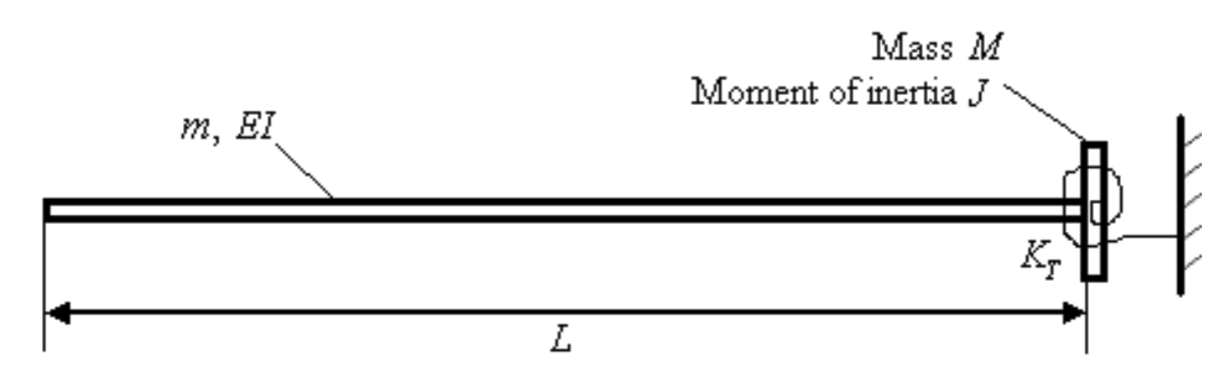
\includegraphics[width=0.7\textwidth]{homework/hw5/assets/hw5_p3_setup.png}
\end{figure}
\begin{enumerate}[(i)]
\item { % 3(i)
    We consider a coordinate $x$ that originates from the left end of the beam ($x = 0$) and extends towards to right end ($x = L$).
    The governing equation and boundary conditions are 
    \begin{subequations}
    \begin{equation}
        EI \frac{\partial^4 u}{\partial x^4}(x, t) + m \frac{\partial^2 u}{\partial t^2}(x, t) = 0, ~~x \in [0, L], ~~ t \geq 0
    \end{equation}
    \begin{equation}
    \begin{gathered}
        EI \frac{\partial^2 u}{\partial x^2}(0, t) = 0, ~~~~ \left[\frac{\partial}{\partial x}\left(EI \frac{\partial^2 u}{\partial x^2}\right) \right](0, t) = 0 \\
        -\left[\frac{\partial}{\partial x}\left(EI \frac{\partial^2 u}{\partial x^2}\right) \right](L, t) + M \frac{\partial^2 u}{\partial t^2}(L, t) = 0 \\
        EI \frac{\partial^2 u}{\partial x^2}(L, t) + K_T \frac{\partial u}{\partial x}(L, t) + J \frac{\partial^3 u}{\partial x^2 \partial t} = 0
    \end{gathered}
    \end{equation}
    \end{subequations}
    Normal mode analysis assumes the separable solution $u(x, t) = \varphi(x) \eta(t)$ where $\eta(t)$ is determined be harmonic with the natural frequency $\omega$. 
    The spatial eigenvalue problem and associated boundary conditions are then 
    \begin{subequations}
    \begin{equation}\label{eqn:hw5_p3_spatial_eqn}
        EI \frac{d^4 \varphi}{d x^4}(x) + \omega^2 m \varphi(x) = 0, ~~x \in [0, L],
    \end{equation}
    \begin{equation}\label{eqn:hw5_p3_bc_left}
        \frac{d^2 \varphi}{d x^2}(0) = 0, ~~~~ \frac{d^3 \varphi}{d x^3}(0) = 0,
    \end{equation}
    \begin{equation}\label{eqn:hw5_p3_bc_right}
    \begin{gathered}
        EI \frac{d^3 \varphi}{dx^3}(L) + \omega^2 M \varphi(L) = 0 \\
        EI \frac{d^2 \varphi}{d x^2}(L) + (K_T - \omega^2 J) \frac{d \varphi}{d x}(L) = 0
    \end{gathered}
    \end{equation}
    \end{subequations}
    Solving \cref{eqn:hw5_p3_spatial_eqn} yields the general solution 
    \begin{equation}
        \varphi(x) = A \cos \frac{\mu x}{L} + B \sin \frac{\mu x}{L} + C \cosh \frac{\mu x}{L} + D \sinh \frac{\mu x}{L}, ~~~~ \mu = \sqrt{\omega} L {\left(\frac{EI}{m}\right)}^{\frac{1}{4}}
    \end{equation}
    Applying the free boundary conditions at $x = 0$ (\cref{eqn:hw5_p3_bc_left}) reveals that $A = C$ and $B = D$. 
    Further imposing the boundary conditions at $x = L$ (\cref{eqn:hw5_p3_bc_right}) leads to the following system 
    \begin{equation}\label{eqn:hw5_p3_eigen_system}
        \underbrace{\begin{bmatrix}
            \mu^2(-c+ch)+\mu\left(\tilde{K}-\mu^4 \tilde{J}\right)(-s+sh) & 
            \mu^2(-s+sh)+\mu\left(\tilde{K}-\mu^4 \tilde{J}\right)(c+ch) \\
            \mu^3(s+sh)+\mu^4\tilde{M}(c+ch) &
            \mu^3(-c+ch)+\mu^4\tilde{M}(s+sh)
        \end{bmatrix}}_{\bt{A}} \begin{bmatrix}
            A \\ B
        \end{bmatrix} = \begin{bmatrix}
            0 \\ 0
        \end{bmatrix}
    \end{equation}
    where we have defined the following dimensionless parameters:
    \begin{equation}
        \tilde{K} := \frac{K_T L}{EI}, ~~~~ \tilde{M} := \frac{M}{mL}, ~~~~ \tilde{J} := \frac{J}{mL^3}
    \end{equation}
    and the following shorthand notations are used for conciseness:
    \begin{equation}
        c := \cos \mu, ~~~~ s := \sin \mu, ~~~~ ch := \cosh \mu, ~~~~ sh := \sinh \mu.
    \end{equation}
    The system \cref{eqn:hw5_p3_eigen_system} requires that $\det \bt{A} = 0$, which permits two scenarios which we discuss below. 
    \begin{enumerate}[(1)]
    \item { % 3(i)(1)
        \emph{$\mu = 0$}. This corresponds to a nontrivial rigid body mode that arises due to the lack of constraint on the beam's displacement (for any solution $\varphi(x)$, $\varphi(x) + \psi$ is also a solution for a non-zero scalar $\psi$). 
    }
    \item { % 3(i)(2)
        \emph{$\mu > 0$}. In this case, we must solve $\det \bt{A} = 0$. 
        After some lengthy algebra, using $c^2 + s^2 = 1$ and $ch^2 - sh^2 = 1$ and dividing the determinant by $2\mu^5 \cosh\mu > 0$, we obtain the frequency equation 
        \begin{equation}\label{eqn:hw5_p3_freq_eqn}
        \begin{aligned}
            v_1(\mu) &= v_2(\mu)\\
            v_1(\mu) &= \cos\mu - \frac{1}{\cosh\mu} \\
            v_2(\mu) &= \mu \tilde{M}(\sin\mu - \cos\mu \tanh\mu) - \frac{1}{\mu}(\tilde{K}-\mu^4 \tilde{J})(\sin\mu + \cos\mu \tanh\mu) \\
            &~~~- \tilde{M}(\tilde{K}-\mu^4 \tilde{J})(\cos\mu + \frac{1}{\cosh\mu}) \\
        \end{aligned}
        \end{equation}
        We note that the $v_2(\mu)$ is regular at $\mu = 0$ with $\lim_{\mu\rightarrow 0} v_2(\mu) = -2(\tilde{M}+1)\tilde{K}$, although it's inconsequential as we assume $\mu > 0$.
        The eigenvalues are obtained by finding the intersections of $v_1(\mu)$ and $v_2(\mu)$. 
        For the parameters tabulated in \cref{tab:hw5_p3_params}, the frequency equation is plotted in \cref{fig:hw5_p3_intersect}. 
        \emph{The first three nonzero, nondimensional natural frequencies are found as $\mu_1 \approx 0.5953$, $\mu_2 \approx 4.3862$, and $\mu_3 \approx 7.3026$.} 
        The eigenfunctions are then 
        \begin{equation}\label{eqn:hw5_p3_eigenfunction}
        \begin{aligned}
            \varphi_n(x) &= A_n \left[\left(\cos\frac{\mu_n x}{L} + \cosh\frac{\mu_n x}{L}\right) \right. \\
            &~~~ - \left.\frac{(\sin\mu_n+\sinh\mu_n) + \mu_n\tilde{M}(\cos\mu_n + \cosh\mu_n)}{(-\cos\mu_n+\cosh\mu_n) + \mu_n\tilde{M}(\sin\mu_n + \sinh\mu_n)} \left(\sin\frac{\mu_n x}{L} + \sinh\frac{\mu_n x}{L}\right)\right]
        \end{aligned}
        \end{equation}
        where $A_n$ is normalized to satisfy the mass-orthonormality condition. 
        For the assumed material parameters, the first three coefficients are $A_1 \approx 0.1607$, $A_2 \approx 0.1865$, and $A_3 \approx 0.1849$.
        \begin{table}
            \centering
            \begin{tabular}{|c|c|c|c|c|c|c|}
                \hline
                $L$ & $E$ & $I$ & $m$ & $M$ & $K_T$ & $J$ \\
                \hline
                \qty{1}{\m} & \qty{70}{\GPa} & \qty{8.33e-6}{\m^4} & \qty{27}{\kg\per\m} & \qty{3}{\kg} & \qty{8}{\kN} & \qty{0.01}{\kg\m\squared}  \\
                \hline
            \end{tabular}
            \caption{Material parameters used for the beam problem. The values are modeled after an aluminum bar with square cross sections.}\label{tab:hw5_p3_params}
        \end{table}
        \begin{figure}[!ht]
            \centering
            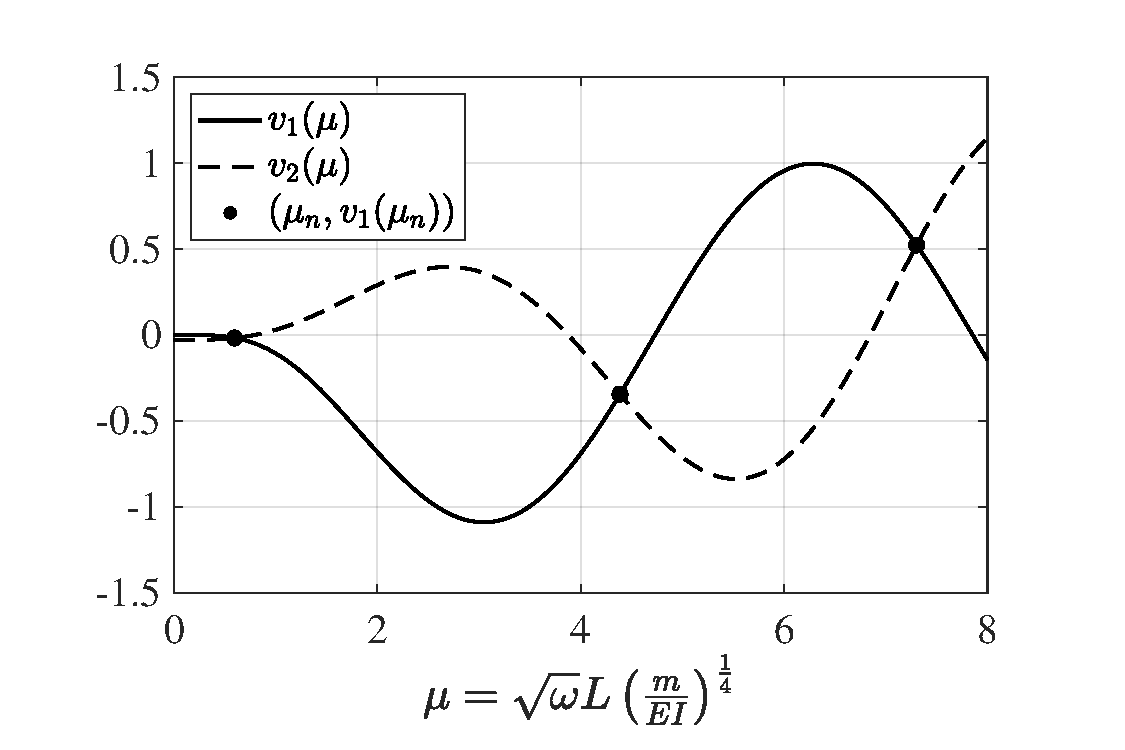
\includegraphics[width=0.6\textwidth]{homework/hw5/assets/hw5_p3_intersect.pdf}
            \caption{Frequency equation \cref{eqn:hw5_p3_freq_eqn} represented as intersections of $v_1(\mu)$ and $v_2(\mu)$.}\label{fig:hw5_p3_intersect}
        \end{figure}
    }
    \end{enumerate}
    The mass- and stiffness-orthonormality conditions are 
    \begin{subequations}
    \begin{equation}\label{eqn:hw5_p3_mass_orthonormality}
        \int_0^L m \varphi_i(x) \varphi_j(x) dx + M \varphi_i(L) \varphi_j(L) + J \varphi_i'(x) \varphi_j'(x) = \delta_{ij} 
    \end{equation}
    \begin{equation}\label{eqn:hw5_p3_stiffness_orthonormality}
        \int_0^L EI \varphi_i''(x) \varphi_j''(x) dx + K_T \varphi_i'(L) \varphi_j'(L) = \omega_i^2 \delta_{ij} 
    \end{equation}
    \end{subequations}
    \newpage
    \begin{prf}{}
        Consider \cref{eqn:hw5_p3_spatial_eqn} for the $i$-th mode $\varphi_i(x)$.
        Taking its inner product with $\varphi_j(x)$ over the domain $[0, L]$, integrating by parts twice, and applying the boundary conditions \cref{eqn:hw5_p3_bc_left,eqn:hw5_p3_bc_right} leads to
        \begin{equation}\label{eqn:hw5_p3_inner_product_1}
        \begin{aligned}
            0 &= \int_0^L \left[EI \frac{d^4 \varphi_i}{d x^4}(x) - \omega_i^2 m \varphi_i(x)\right] \varphi_j(x) dx \\
            &= {\left[EI \varphi_i'''\varphi_j - EI\varphi_i'' \varphi_j' \right]}_0^L + \int_0^L EI\varphi_i'' \varphi_j'' dx - \omega_i^2 \int_0^L m \varphi_i \varphi_j dx \\
            &= \int_0^L EI\varphi_i'' \varphi_j'' dx + K_T \varphi_i'(L) \varphi_j'(L) - \omega_i^2 \left[ \int_0^L m \varphi_i \varphi_j dx + M \varphi_i(L) \varphi_j(L) + J \varphi_i'(L) \varphi_j'(L)\right]
        \end{aligned}
        \end{equation}
        A similar equation can be obtained by switching the indices $i$ and $j$:
        \begin{equation}\label{eqn:hw5_p3_inner_product_2}
            0 = \int_0^L EI\varphi_i'' \varphi_j'' dx + K_T \varphi_i'(L) \varphi_j'(L) - \omega_j^2 \left[ \int_0^L m \varphi_i \varphi_j dx + M \varphi_i(L) \varphi_j(L) + J \varphi_i'(L) \varphi_j'(L)\right]
        \end{equation}
        Subtracting \cref{eqn:hw5_p3_inner_product_2} from \cref{eqn:hw5_p3_inner_product_1} eliminates the stiffness terms and, given $\omega_i \neq \omega_j$ for $i \neq j$, leads to the mass-orthonormality condition \cref{eqn:hw5_p3_mass_orthonormality}.
        Substituting the mass-orthonormality back into \cref{eqn:hw5_p3_inner_product_1} results in the stiffness-orthonormality condition \cref{eqn:hw5_p3_stiffness_orthonormality}.
    \end{prf}
}
\item { % 3(ii)
    First, we note that the system always has a rigid-body mode. However, this DOF corresponds to constant displacement of the entire beam but is not associated with oscillations. 
    Thus, in this context we tentatively consider this DOF trivial and seek an additional DOF that results in oscillations. 
    
    Regarding the three nondimensional parameters $\tilde{K}$, $\tilde{J}$, and $\tilde{M}$, several limiting cases lead to additional DOFs. 
    However, the one that corresponds to a single-DOF oscillation is \emph{$\tilde{J} \rightarrow \infty$, or $J \gg mL^3$}. 
    Intuitively, this means that the system is dominated by the the rotational inertia of the trailing mass and behaves as if only the mass is oscillating angularly under the torsional spring force. 
    To see this more concretely, we return to the frequency equation \cref{eqn:hw5_p3_freq_eqn} and use the following asymptotic behaviors for small $\mu$:
    \begin{equation}
        \sin\mu = \mu + \order{\mu^3}, ~~ \cos\mu = 1 + \order{\mu^2}, ~~ \cosh\mu = 1 + \order{\mu^2}, ~~ \tanh\mu = \mu + \order{\mu^3}
    \end{equation}
    and find that 
    \begin{equation}
        v_1(\mu) \sim 0, ~~~~ v_2(\mu) \sim -2(\tilde{M}+1)\tilde{K} + 2(\tilde{M}+1)\tilde{J}\mu^4
    \end{equation}
    where the 4th-degree terms are not dropped due to $\tilde{J}$ being arbitrarily large.
    Equating $v_1$ and $v_2$ permits a near-zero natural frequency $\mu \approx {(\tilde{K} / \tilde{J})}^{1/4}$.
    Hence, 
    \begin{equation}
        \omega = \frac{\mu^2}{L^2}\sqrt{\frac{EI}{m}} \approx  \sqrt{\frac{EI\tilde{K}}{mL^4\tilde{J}}} = \sqrt{\frac{K_T}{J}}
    \end{equation}
    which is the natural frequency of the mass with moment of inertia $J$ oscillating with the torsional spring with stiffness $K_T$. 
}
\item { % 3(iii)
    Given an admissable trial function $\tilde{\varphi}(x)$, the Rayleigh quotient is 
    \begin{equation}
        R[\tilde{\varphi}(x)] := \frac{
            \int_0^L EI {[\tilde{\varphi}''(x)]}^2 dx + K_T {[\tilde{\varphi}'(L)]}^2
        }{
            \int_0^L m {\tilde{\varphi}(x)}^2 dx + M {\tilde{\varphi}(L)}^2 + J {[\tilde{\varphi}'(L)]}^2
        }
    \end{equation}
    Estimation of the first natural frequency is relayed to the discussion in (iv). 
}
\item { % 3(iv)
    For the Rayleigh-Ritz approximation, we elect to use the finite element formulation where we segment the integral on $[0, L]$ into $N_e$ uniform sub-domains $\Omega^e$, $e = 1, 2, \ldots, N_e$. 
    On each sub-domain we use 4 basis functions transformed from the reference domain $\xi \in [-1, 1]$, which are discussed in lectures as the ``influence functions'':
    \begin{equation}
    \begin{aligned}
        N_1(\xi) &= \frac{1}{4}(\xi^3 - 3\xi + 2) \\
        N_2(\xi) &= \frac{1}{4}(\xi^3-\xi^2-\xi+1) \\
        N_3(\xi) &= \frac{1}{4}(-\xi^3+3\xi+2) \\
        N_4(\xi) &= \frac{1}{4}(\xi^3+\xi^2-\xi-1)
    \end{aligned}
    \end{equation}
    Each domain boundary (node) is attached two scalar nodal values $u_i$ and $\theta_i$, $i = 0, 1, \ldots, N_e$ such that the displacement field within each sub-domain is approximated as 
    \begin{equation}\label{eqn:hw5_p3_synthesis}
        u(x) = N_1(\xi(x)) u_{e1} + N_2(\xi(x)) \theta_{e1} + N_3(\xi(x)) u_{e2} + N_4(\xi(x)) \theta_{e2}
    \end{equation}
    where $\xi(x)$ maps the physical coordinate $x$ to the reference coordinate $\xi$ for each $\Omega^e$, and the scalars with double subscripts are mapped to nodal values during assembly (e.g. $u_{e2}$ is the same as $u_{e}$ in the global numbering). 
    The elemental mass and stiffness matrices are 
    \begin{equation}
        \bt{M}^e = \frac{1}{105}\begin{bmatrix}
            78  & 22 & 27  & -13 \\
            22  & 8  & 13  & -6  \\
            27  & 13 & 78  & -22 \\
            -13 & -6 & -22 & 8 
        \end{bmatrix}, ~~~~ 
        \bt{K}^e = \frac{1}{2}\begin{bmatrix}
            3  & 3 & -3 & 3  \\
            3  & 4 & -3 & 2  \\
            -3 & 3 & 3  & -3 \\
            3  & 2 & -3 & 4
        \end{bmatrix}
    \end{equation}
    Let $j = dx / d\xi = L / 2N_e$ be the Jacobian for each element. 
    The Rayleigh quotient is then 
    \begin{equation}
        R = \frac{
            \sum_{e=1}^{N_e} j^{-3}{(\bv{u}^e)}^T \bt{K}^e (\bv{u}^e) + j^{-2} K_T \theta_{N_e}^2
        }{
            \sum_{e=1}^{N_e} j{(\bv{u}^e)}^T \bt{M}^e (\bv{u}^e) + M u_{N_e}^2 + j^{-2} J \theta_{N_e}^2
        } = \frac{\bv{u}^T \bt{K} \bv{u}}{\bv{u}^T \bt{M} \bv{u}}
    \end{equation}
    where 
    \begin{equation}
        \bv{u_e} = \begin{bmatrix}
            u_{e1} \\ \theta_{e1} \\ u_{e2} \\ \theta_{e2}
        \end{bmatrix} = \begin{bmatrix}
            u_{e-1} \\ \theta_{e-1} \\ u_{e} \\ \theta_{e}
        \end{bmatrix}
    \end{equation}
    One can assemble the elemental matrices into the global discretized eigenvalue problem $\bt{K}\bv{u} = \omega^2 \bt{M} \bv{u}$. 

    For this problem, we estimate the eigenpairs with 8 uniform elements ($N_e = 8$), which totals to $18$ degrees of freedoms (9 displacements and 9 rotations).
    \emph{The computed (non-zero) natural frequencies are $\mu_1 \approx 0.5953$, $\mu_2 \approx 4.3862$, and $\mu_3 \approx 7.3026$, consistent with those obtained analytically in (i).}
    The mass-orthonormalized eigenfunctions are obtained through synthesis \cref{eqn:hw5_p3_synthesis} with nodal coefficients $u_e, \theta_e, e = 0, \ldots N_e$, as tabulated in \cref{tab:hw5_p3_data}.
    The eigenfunctions are plotted in \cref{fig:hw5_p3_eigfunc} for comparison with the analytical solution \cref{eqn:hw5_p3_eigenfunction}, noting good quantitative agreement. 

    \begin{table}[!ht]
    \centering
    \begin{tabular}{|c|c|c|c|c|c|c|}
        \hline 
        Index & \multicolumn{2}{|c|}{$\varphi_1(x)$} & \multicolumn{2}{|c|}{$\varphi_2(x)$} & \multicolumn{2}{|c|}{$\varphi_3(x)$} \\ \hline 
        $e$ & $u_e$ & $\theta_e$ & $u_e$ & $\theta_e$ & $u_e$ & $\theta_e$ \\ \hline
        0 & -0.3213 & 0.0366 &  0.3730 & -0.1006 &  0.3701 & -0.1690 \\ \hline
        1 & -0.2482 & 0.0365 &  0.1731 & -0.0982 &  0.0407 & -0.1525 \\ \hline
        2 & -0.1751 & 0.0365 & -0.0117 & -0.0841 & -0.1965 & -0.0742 \\ \hline
        3 & -0.1021 & 0.0365 & -0.1532 & -0.0549 & -0.2321 &  0.0386 \\ \hline
        4 & -0.0290 & 0.0365 & -0.2235 & -0.0142 & -0.0693 &  0.1114 \\ \hline
        5 &  0.0440 & 0.0365 & -0.2078 &  0.0296 &  0.1504 &  0.0918 \\ \hline
        6 &  0.1169 & 0.0364 & -0.1098 &  0.0665 &  0.2443 & -0.0062 \\ \hline
        9 &  0.1897 & 0.0364 &  0.0489 &  0.0896 &  0.1192 & -0.1139 \\ \hline
        8 &  0.2624 & 0.0363 &  0.2380 &  0.0973 & -0.1739 & -0.1680 \\ \hline
    \end{tabular}
    \caption{Rayleigh-Ritz approximated nodal values of the first three eigenfunctions. The full eigenfunctions are synthesized using the basis functions as in \cref{eqn:hw5_p3_synthesis}.}\label{tab:hw5_p3_data}
    \end{table}
    \begin{figure}[!ht]
        \centering
        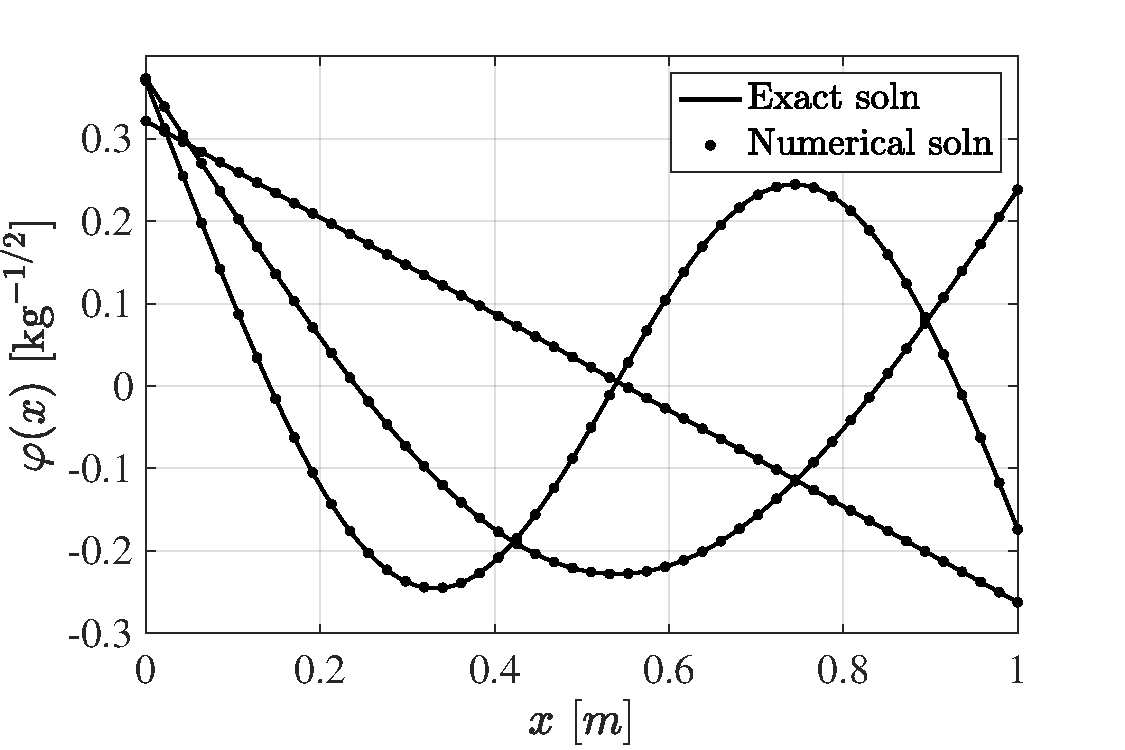
\includegraphics[width=0.52\textwidth]{homework/hw5/assets/hw5_p3_eigfunc.pdf}
        \caption{Comparison of the first three mass-orthonormalized eigenfunctions between the analytical solution \cref{eqn:hw5_p3_eigenfunction} and numerically computed values \cref{tab:hw5_p3_data}. The MATLAB code for this problem can be found at \url{https://github.com/sy-cui/TAM514/blob/main/latex/homework/hw5/assets/hw5_p3.m}. }\label{fig:hw5_p3_eigfunc}
    \end{figure}
    
}
\end{enumerate}

\newpage
\begin{problem}
    \textbf{4 (200 pts).} 
    Given, 
    \begin{equation}\label{eqn:hw5_p4_gov_eqns}
    \begin{gathered}
        u_{xx} - [1 + \varepsilon \alpha(x)]u_{tt} = 0, ~~ 0 \leq x \leq 1 \\
        u(0, t) = u(1, t) = 0 \\
    \end{gathered}
    \end{equation}
    where $0 < \varepsilon \ll 1$ is a small parameter, and $\alpha(x) = A\sin(\pi x / 2)$ is a smooth function.
    Compute the first order analytical approximation of the eigensolution of this problem by means of a
    perturbation approach.
    \begin{enumerate}[(i)]
        \item {
            Introduce a space-time separation by expressing the solution as $u(x, t) = \varphi(x) e^{j\omega t}$.
        }
        \item {
            Solve approximately the resulting eigenvalue problem governing $\varphi(x)$ by expressing the solution in the form $\varphi(x) = \varphi_0(x) + \varepsilon \varphi_1(x) + \ldots$, expanding also the frequency in the form $\omega(x) = \omega_0(x) + \varepsilon \omega_1(x) + \ldots$ and substituting into the eigenvalue problem.
        }
        \item {
            By grouping terms of \order{1} and \order{\varepsilon} obtain the two eigenvalue subproblems that govern the leading-order approximations. 
        }
        \item {
            Solve these eigenvalue subproblems to obtain an analytic approximation for the eigensolution of the original problem correct to \order{\varepsilon}. 
            Orthonormalize the approximations derived for the eigenfunctions.
        }
    \end{enumerate}
\end{problem}

\begin{enumerate}[(i)]
\item { % 4(i)
    By setting $u(x, t) = \varphi(x) e^{j\omega t}$ and cancelling the temporally oscillatory term $e^{j\omega t}$ the PDE \cref{eqn:hw5_p4_gov_eqns} becomes 
    \begin{equation}\label{eqn:hw5_p4_spatial_gov_eqn}
        \frac{d^2 \varphi}{dx^2}(x) + \left[1 + \varepsilon \alpha(x)\right] \omega^2 \varphi(x) = 0
    \end{equation}
    subject to the boundary conditions 
    \begin{equation}
        \varphi(0) = \varphi(1) = 0.
    \end{equation}
    This transforms the spatio-temporal PDE into a space-only modal equation. 
}
\item { % 4(ii)
    Consider the asymptotic expansion 
    \begin{equation}
        \varphi(x) = \varphi_0(x) + \varepsilon \varphi_1(x) + \ldots, ~~~~ 
        \omega = \omega_0 + \varepsilon \omega_1 + \ldots.
    \end{equation}
    Substituting into \cref{eqn:hw5_p4_spatial_gov_eqn} yields 
    \begin{equation}\label{eqn:hw5_p4_gov_asymp}
    \begin{aligned}
        0 &= \left[\varphi_0''(x) + \varepsilon \varphi_1''(x) + \ldots \right] + \left[1 + \varepsilon \alpha(x)\right] \left[\omega_0^2 + 2 \varepsilon \omega_0\omega_1 + \ldots \right] \left[\varphi_0(x) + \varepsilon \varphi_1(x) + \ldots \right]  \\
        &= \varphi_0''(x) + \omega_0^2 \varphi_0(x) + \varepsilon \left[\varphi_1''(x) + 2\omega_0\omega_1 \varphi_0(x) + \omega_0^2 \varphi_1(x) + \alpha(x) \omega_0^2 \varphi_0(x)\right] + \order{\varepsilon^2} \\
    \end{aligned}
    \end{equation}
    The boundary conditions are 
    \begin{equation}\label{eqn:hw5_p4_bc_asymp}
        \varphi_0(0) + \varepsilon \varphi_1(0) + \cdots = \varphi_0(1) + \varepsilon \varphi_1(1) + \cdots = 0.
    \end{equation}
}
\item { % 4(iii)
    The \order{1} equation and boundary conditions, based on \cref{eqn:hw5_p4_gov_asymp,eqn:hw5_p4_bc_asymp}, are 
    \begin{equation}\label{eqn:hw5_p4_gov_0}
        \varphi_0''(x) + \omega_0^2 \varphi_0(x) = 0, ~~~~ 
        \varphi_0(0) = \varphi_0(1) = 0.
    \end{equation}
    The \order{\varepsilon} equation and boundary conditions for each of $n = 1, 2, \ldots$ read
    \begin{equation}\label{eqn:hw5_p4_gov_1}
        \frac{d^2 \varphi_1^n(x)}{dx^2} + {(\omega_0^n)}^2 \varphi_1^n(x) = -2\omega_0^n \omega_1^n \varphi_0^n(x) - \alpha(x) {(\omega_0^n)}^2 \varphi_0^n(x), ~~~~ \varphi_1^n(0) = \varphi_1^n(1) = 0.
    \end{equation}
}
\item { % 4(iv)
    \Cref{eqn:hw5_p4_gov_0} has orthonormalized eigensolutions 
    \begin{equation}
        \varphi_0^{n}(x) = \sqrt{2} \sin\omega_0^{n} x, ~~~~
        \omega_0^{n} = n\pi, ~~~~ n = 1, 2, \ldots
    \end{equation}
    where we use superscripts to denote the countably-infinite number of eigenmodes. 
    The eigenmodes satisfy the orthonormality condition
    \begin{equation}
        \int_0^1 \varphi_0^n(x) \varphi_0^m(x) dx = \delta_{nm}
    \end{equation}
    Since $\varphi_0^n(x)$ forms a complete orthonormal basis on $[0, 1]$ with the given boundary conditions, we write 
    \begin{equation}
        \varphi_1^n(x) = \sum_{k=1}^\infty C_{nk} \varphi_0^k(x), ~~~~ C_{nk} = \int_0^1 \varphi_0^k(x) \varphi_1^n(x) dx.
    \end{equation}
    Substituting into \cref{eqn:hw5_p4_gov_1} and taking the inner product with $\varphi_0^m(x)$ (for some $m=1,2,\ldots$) leads to 
    \begin{subequations}
    \begin{align}
    \begin{split}
        \textrm{LHS} &= \sum_{k=1}^\infty C_{nk} \int_0^1 \frac{d^2 \varphi_0^k(x)}{dx^2} \varphi_0^m(x) dx + {(\omega_0^n)}^2 \sum_{k=1}^\infty C_{nk} \int_0^1 \varphi_0^k(x) \varphi_0^m(x) dx \\
        &= \sum_{k=1}^\infty C_{nk} \left[{(\omega_0^n)}^2 - {(\omega_0^k)}^2 \right] \int_0^1 \varphi_0^k(x) \varphi_0^m(x) dx \\
        &= C_{nm} \left[{(\omega_0^n)}^2 - {(\omega_0^m)}^2 \right]
    \end{split} \\
    \begin{split}
        \textrm{RHS} &= -2\omega_0^n \omega_1^n \int_0^1 \varphi_0^n(x) \varphi_0^m(x) dx - {(\omega_0^n)}^2 \int_0^1 \alpha(x) \varphi_0^n(x) \varphi_0^m(x) dx \\
        &= -2\omega_0^n \omega_1^n \delta_{nm} - {(\omega_0^n)}^2 \int_0^1 \alpha(x) \varphi_0^n(x) \varphi_0^m(x) dx
    \end{split}
    \end{align}
    \end{subequations}
    where for the left-hand side we have used \cref{eqn:hw5_p4_gov_0} to remove the derivatives.
    The goal is to find the coefficients $C_{nm}$ as well as the first-order eigenvalues $\omega_1^n$. 
    In particular, the integral is evaluated as 
    \begin{equation}
    \begin{aligned}
        v_{nm} 
        &= \int_0^1 \alpha(x) \varphi_0^n(x) \varphi_0^m(x) dx \\
        &= 2A \int_0^1 \sin\left(\frac{\pi x}{2}\right) \sin\left(n\pi x\right) \sin\left(m\pi x\right) dx \\
        &= \frac{A}{2} \int_0^1 \left\{
            \sin\left[\left(\frac{1}{2}+n-m\right)\pi x\right]+  
            \sin\left[\left(\frac{1}{2}-n+m\right)\pi x\right]-
        \right. \\ & \qquad \qquad ~~ \left.
            \sin\left[\left(\frac{1}{2}+n+m\right)\pi x\right]-
            \sin\left[\left(\frac{1}{2}-n-m\right)\pi x\right]
            \right\} dx \\
        &= \frac{A}{\pi} \left(\frac{1}{1+2n-2m} + \frac{1}{1-2n+2m} - \frac{1}{1+2n+2m} - \frac{1}{1-2n-2m}\right) \\
        &=\frac{-32 A nm}{\pi\left[1 - 4{(n-m)}^2\right] \left[1 - 4{(n+m)}^2\right]}
    \end{aligned}
    \end{equation}
    Hence, setting $\textrm{LHS} = \textrm{RHS}$ results in the equation
    \begin{equation}
        C_{nm} \left[{(\omega_0^n)}^2 - {(\omega_0^m)}^2 \right] = -2\omega_0^n \omega_1^n \delta_{nm} - {(\omega_0^n)}^2 v_{nm}.
    \end{equation}
    Considering the two cases $n = m$ and $n \neq m$ leads to the following observations
    \begin{equation}
        \begin{cases}
            C_{nm} = \dfrac{{(\omega_0^n)}^2}{{(\omega_0^m)}^2 - {(\omega_0^n)}^2} v_{nm} = \dfrac{32 A n^3 m}{\pi(n^2 - m^2)\left[1 - 4{(n-m)}^2\right] \left[1 - 4{(n+m)}^2\right]}, & n \neq m \\
            \omega_1^n = \dfrac{-\omega_0^n}{2}v_{nn}  = \dfrac{16 A n^3}{1 - 16n^2}, & n = m
        \end{cases}
    \end{equation}
    Furthermore, we impose the orthonormality condition on the full eigenfunction 
    \begin{equation}
    \begin{aligned}
        0 &= \int_0^1 
        \left[\varphi_0^n(x) + \varepsilon \varphi_1^n(x) + \cdots \right] 
        \left[\varphi_0^m(x) + \varepsilon \varphi_1^m(x) + \cdots \right] 
        \left[1 + \varepsilon \alpha(x) \right] dx - \delta_{nm} \\
        &= 
        \left[\int_0^1 \varphi_0^n(x) \varphi_0^m(x) dx - \delta_{nm}\right] 
        + \varepsilon \int_0^1 \left[\varphi_0^n(x) \varphi_1^m(x) + \varphi_1^n(x) \varphi_0^m(x) + \alpha(x) \varphi_0^n(x) \varphi_0^m(x) \right] dx 
        + \order{\varepsilon^2} \\
        &= \int_0^1 \left[\varphi_0^n(x) \varphi_1^m(x) + \varphi_1^n(x) \varphi_0^m(x) + \alpha(x) \varphi_0^n(x) \varphi_0^m(x)\right] dx \\
        &= C_{mn} + C_{nm} + v_{nm}
    \end{aligned}
    \end{equation}
    which implies that the diagonal terms are
    \begin{equation}
        C_{nn} = -\frac{1}{2}v_{nn} = \frac{16 A n^2}{\pi(1 - 16n^2)}.
    \end{equation}

    To summarize, the first-order approximation of the eigensolution is 
    \begin{equation}\label{eqn:hw5_p4_soln}
    \begin{aligned}
        \omega^n &= n\pi + \varepsilon \frac{16 A n^3}{1 - 16n^2} + \order{\varepsilon^2} \\
        \varphi^n(x) &= \sqrt{2} \sin(n\pi x) + \varepsilon \sum_{k=1}^\infty C_{nk} \sqrt{2} \sin(k\pi x)  + \order{\varepsilon^2} \\
        C_{nk} &= \begin{cases}
            \frac{16 A n^2}{\pi(1 - 16n^2)} & n = k \\
            \frac{32 A n^3 k}{\pi(n^2 - k^2)\left[1 - 4{(n-k)}^2\right] \left[1 - 4{(n+k)}^2\right]}, & n \neq k
        \end{cases}
    \end{aligned}
    \end{equation}
    See \cref{fig:hw5_p4_conv} for the mode shapes and further analytics.
}
\begin{figure}[!ht]
    \centering
    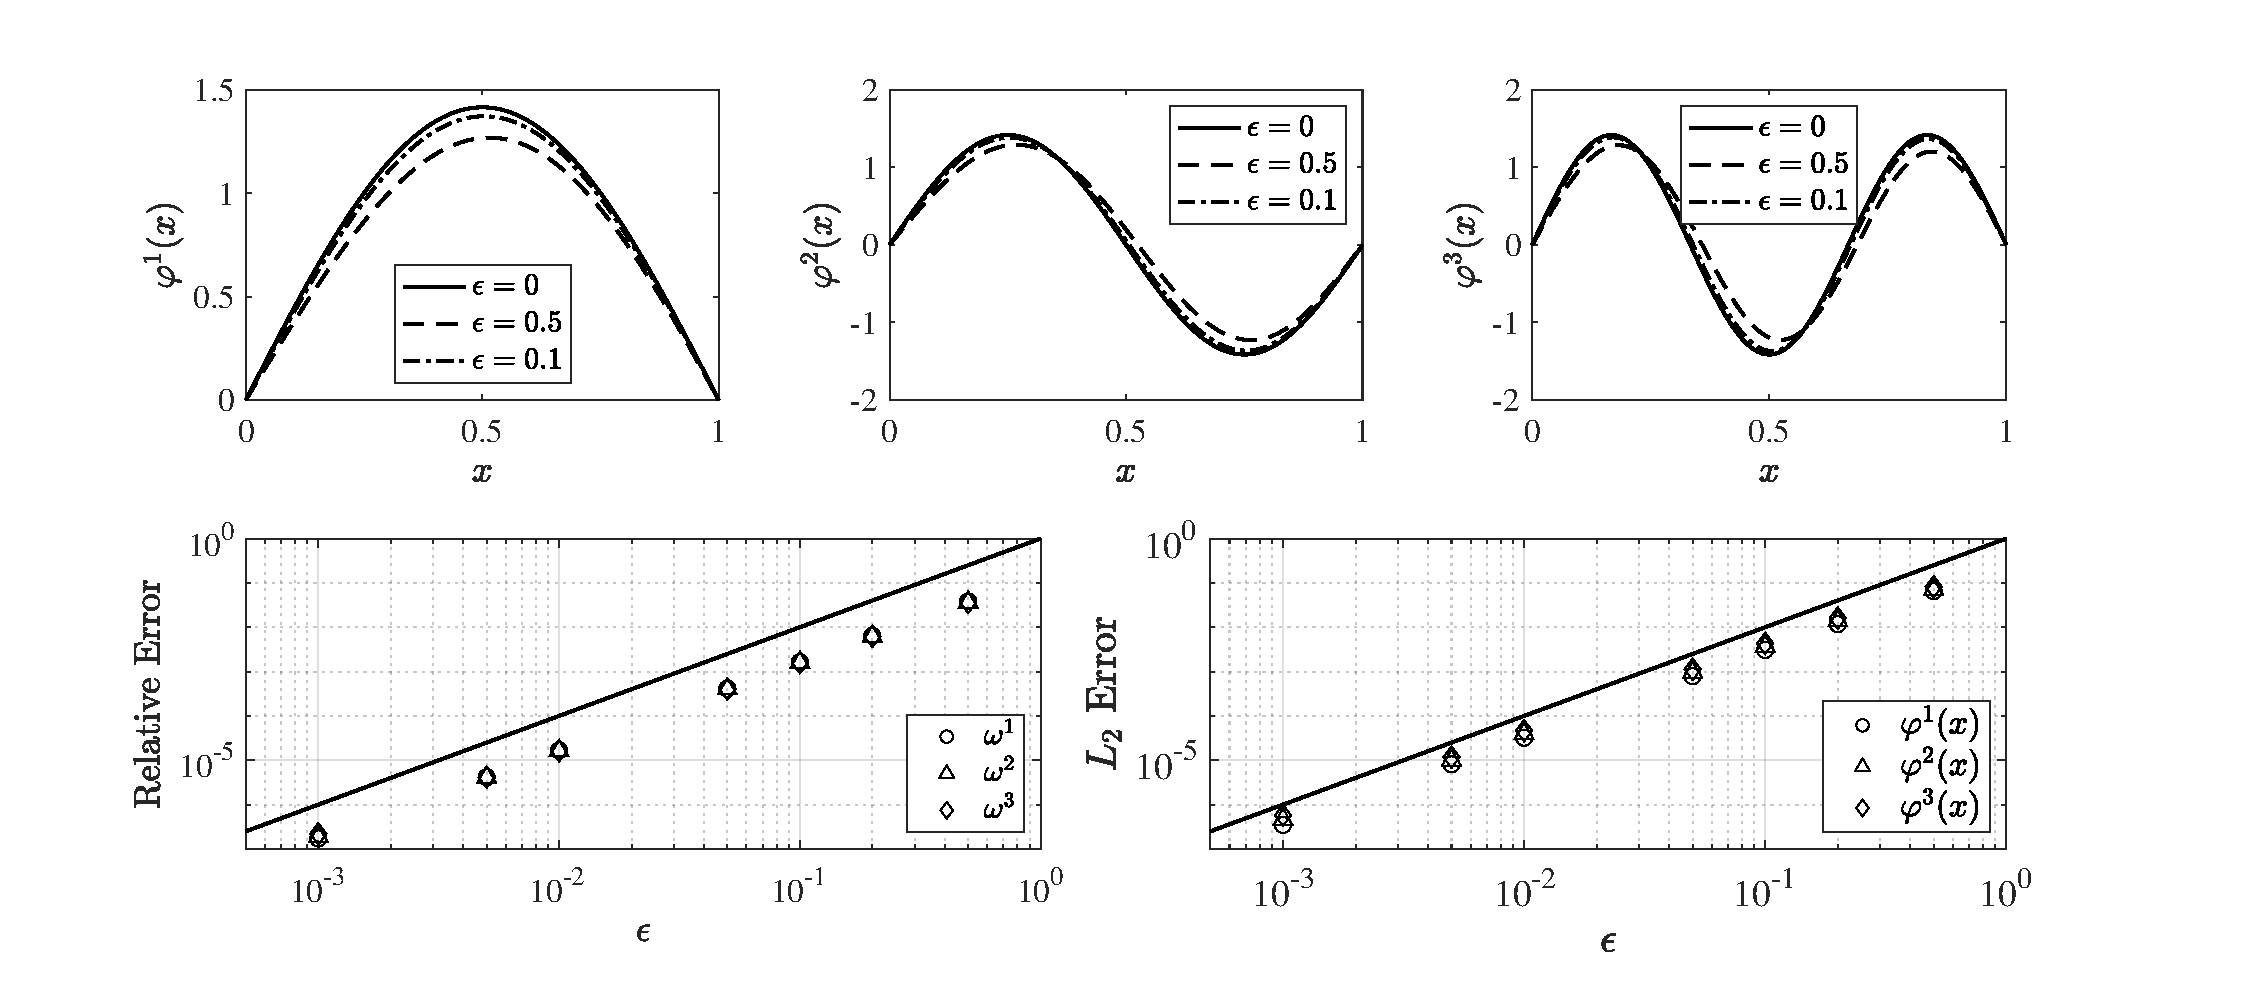
\includegraphics[width=\textwidth]{homework/hw5/assets/hw5_p4_conv.pdf}
    \caption{
        First three orthonormalized mode shapes (upper row) for various $\epsilon$ values, and the error convergence of the natural frequencies and eigenfunctions compared with finite element solutions (lower row). 
        Without loss of generality, $A = 1$ is used for all tests. 
        The truncated ($k \leq 50$) asymptotic solutions \cref{eqn:hw5_p4_soln} for $\varepsilon = 0$, $\varepsilon = 0.1$, and $\varepsilon = 0.5$ are plotted for the first three modes. 
        The solution for more $\varepsilon$ values are compared against those obtained through finite element modeling using 8192 uniform elements with piecewise linear basis functions and sufficiently high quadrature orders. 
        This ensures the numerical error is negligible in the inspected range (no more than $10^{-7}$). 
        Shown in the lower left plot, the error in natural frequency is computed as $e_i = |\omega^n - \tilde{\omega}^n| / \tilde{\omega}^n$ with $\tilde{\omega}^n$ being the $n$-th numerically computed natural frequency. 
        The lower right plot shows the $L_2$ error norm of the first three orthonormalized eigenfunctions. 
        \emph{The solid black lines in the lower two plots represent $\varepsilon^2$ which is the expected rate of convergence for a first-order asymptotic approximation.} 
        The MATLAB code for this problem can be found at \url{https://github.com/sy-cui/TAM514/blob/main/latex/homework/hw5/assets/hw5_p4.m}.
        An alternative Rayleigh-Ritz approximation using spectral methods can be found at \url{https://github.com/sy-cui/TAM514/blob/main/latex/homework/hw5/assets/hw5_p4_spectral.m}.
    }\label{fig:hw5_p4_conv}
\end{figure}

\end{enumerate}

\begin{problem}
    \textbf{5 (100 pts).}
    The dynamics of a long bridge due to a crossing locomotive is described approximately by the following equation,
    \begin{equation}
    \begin{gathered}
        EIu_{xxxx} + cu_t + mu_{tt} = (M_1 + \omega^2 M_2 \cos\omega t) \delta(x - Vt), ~~ 0 \leq x \leq L, ~~ t \geq 0 \\
        u(0, t) = u(L, t) = u_{xx}(0, t) = u_{xx}(L, t) = 0 \\
    \end{gathered}
    \end{equation}
    where $M_1$ is the mass of the locomotive, $M_2$ the mass of the unbalanced rotating and reciprocating parts with $\omega$ being the frequency of rotation in (\si{\radian\per\s}) of the drive wheels, and $V$ is the forward velocity of the locomotive. 
    Assume that the bridge is underdamped.
    \begin{enumerate}[(i)]
        \item {
            Solve this problem assuming that the bridge is at rest when the train enters.
        }
        \item {
            Under what conditions can resonance occur, and the bridge be in danger?
        }
    \end{enumerate}
\end{problem}
\emph{Possibly due to some unspecified assumptions, the right-hand side appears dimensionally inconsistent. 
We shall assume ($M_1 + \omega^2 M_2 \cos\omega t$) to be of force units (e.g. Newtons).}
\begin{enumerate}[(i)]
\item { % 5(i)
    Normal mode analysis assumes the separable solution $u(x, t) = \varphi(x) \eta(t)$, which is substituted into the unforced governing equation to separate the spatial and temporal equations:
    \begin{subequations}
    \begin{align}
        \label{eqn:hw5_p5_spatial_eqn} EI \frac{d^4 \varphi(x)}{dx^4} - m \Omega^2 \varphi(x) &= 0 \\ 
        \frac{d^2 \eta(t)}{dt^2} + c \frac{d\eta(t)}{dt} + m \Omega^2 \eta(t) &= 0
    \end{align}
    \end{subequations}
    where $\Omega$ is the natural frequency. 
    \Cref{eqn:hw5_p5_spatial_eqn} must also satisfy the boundary conditions 
    \begin{equation}
        \varphi(0) = \varphi(L) = 0, ~~~~ \varphi''(0) = \varphi''(L) = 0
    \end{equation}
    The mass-orthonormal modal solution to this double-simply-supported beam is 
    \begin{equation}
        \varphi_n(x) = \sqrt{\frac{2}{mL}} \sin \left(\mu_n \frac{x}{L}\right), ~~~~ \mu_n = \sqrt{\Omega_n} L {\left(\frac{m}{EI}\right)}^{\frac{1}{4}} = n\pi
    \end{equation}
    for countably-infinite $n = 1, 2, \ldots$.
    The mass-orthonormality condition is readily satisfied:
    \begin{equation}\label{eqn:hw5_p5_mass_orthonormality}
        \int_0^L m \varphi_i(x) \varphi_j(x) dx = \delta_{ij}.
    \end{equation}
    Next, we substitute the superposition of modes $u(x, t) = \sum_{j=1}^\infty \varphi_j(x) \eta_j(t)$ into the \emph{forced} equation, take inner products with $\varphi_n(x)$, $n = 1, 2, \ldots$ over $[0, L]$, and apply \cref{eqn:hw5_p5_mass_orthonormality} to obtain the temporal modal oscillators:
    \begin{equation}\label{eqn:hw5_p5_modal_oscillators}
    \begin{aligned}
        \ddot{\eta}_n(t) + \frac{c}{m} \dot{\eta}_n(t) + \Omega_n^2 \eta_n(t) &= \int_0^L \varphi_n(x) \left[(M_1 + \omega^2 M_2 \cos\omega t) \delta(x - Vt)\right] dx \\
        &= \sqrt{\frac{2}{mL}} \sin \left( n \pi \frac{Vt}{L} \right) (M_1 + \omega^2 M_2 \cos\omega t) \\
        &= M_1 \sqrt{\frac{2}{mL}} \sin \left(\frac{n\pi V}{L}t\right) + \frac{\omega^2 M_2}{2}\sqrt{\frac{2}{mL}} \left\{\sin \left[\left(\frac{n\pi V}{L} + \omega\right) t\right] \right. \\
        &~~~+ \left. \sin \left[\left(\frac{n\pi V}{L} - \omega\right) t\right] \right\}
    \end{aligned}
    \end{equation}
    The homogeneous solution is 
    \begin{equation}
        \eta_n^h(t) = e^{-\zeta t} \left(A_n \cos \eta_n t + B_n \sin \eta_n t \right)
    \end{equation}
    where we have defined 
    \begin{equation}
        \zeta := \frac{c}{2m}, ~~~~ \eta_n := \sqrt{\Omega_n^2 - \zeta^2}.
    \end{equation}
    The system is assumed to be underdamped, which means even the first mode still has oscillatory component ($\zeta < \Omega_1$ and $\eta_n \in \mathbb{R}$). 
    To find the inhomogeneous solution of \cref{eqn:hw5_p5_modal_oscillators}, we consider the following model problem:
    \begin{equation}\label{eqn:hw5_p5_model_problem}
        \ddot{\eta}_n(t) + 2\zeta \dot{\eta}_n(t) + \Omega_n^2 \eta_n(t) = \sin \sigma t
    \end{equation}
    where $\sigma$ is the forcing frequency. 
    \emph{Resonance occurs when $\sigma = \eta_n$, which we assume to not be the case for now. }
    This allows the ansatz $\eta_n(t) = C_n \cos\sigma t + D_n \sin\sigma t$, which is substituted into \cref{eqn:hw5_p5_model_problem} to yield the following system:
    \begin{equation}
        \begin{bmatrix}
            \Omega_n^2 - \sigma^2 & 2\zeta \sigma \\
            -2\zeta \sigma & \Omega_n^2 - \sigma^2
        \end{bmatrix} \begin{bmatrix}
            C_n \\ D_n
        \end{bmatrix} = \begin{bmatrix}
            0 \\ 1
        \end{bmatrix}
    \end{equation}
    The coefficients $C_n$ and $D_n$ are obtained by solving the system, and the inhomogeneous solution to \cref{eqn:hw5_p5_model_problem} is then 
    \begin{equation}
        \eta_n^p(t) = \frac{1}{{(\Omega_n^2 - \sigma^2)}^2 + 4\zeta^2 \sigma^2} \left[(\Omega_n^2 - \sigma^2) \sin\sigma t - 2 \zeta \sigma \cos\sigma t \right]
    \end{equation}
    This template can be applied to the RHS terms of \cref{eqn:hw5_p5_modal_oscillators} to obtain the full non-resonant solution.
    \begin{equation}
    \begin{aligned}
        \eta_n(t) = \tilde{\eta}_n(\tau) &= e^{-\gamma \tau} \left[A_n \cos \sqrt{\alpha_n^2 - \gamma^2} \tau + B_n \sin \sqrt{\alpha_n^2 - \gamma^2} \tau\right] \\
        &~~~ +\frac{M_1}{\omega^2} \sqrt{\frac{2}{mL}} \frac{
            \left(\alpha_n^2 -\beta^2\right)\sin \beta \tau - 2\beta\gamma\cos \beta \tau
        }{
            {\left(\alpha_n^2 - \beta^2\right)}^2 + 4\beta^2\gamma^2
        } \\
        &~~~ + \frac{M_2}{2}\sqrt{\frac{2}{mL}} \frac{
            \left[\alpha_n^2 - {(\beta + 1)}^2 \right]\sin (\beta + 1) \tau 
            - 2\gamma(\beta + 1)\cos (\beta + 1) \tau
        }{
            {\left[\alpha_n^2 - {(\beta + 1)}^2 \right]}^2 + 4\gamma^2 {(\beta + 1)}^2
        } \\ 
        &~~~ + \frac{M_2}{2}\sqrt{\frac{2}{mL}} \frac{
            \left[\alpha_n^2 - {(\beta - 1)}^2 \right]\sin (\beta - 1) \tau 
            - 2\gamma(\beta - 1)\cos (\beta - 1) \tau 
        }{
            {\left[\alpha_n^2 - {(\beta - 1)}^2 \right]}^2 + 4\gamma^2 {(\beta - 1)}^2
        } \\ 
    \end{aligned}
    \end{equation}
    where the following non-dimensional parameters are used:
    \begin{equation}
        \alpha_n = \frac{\Omega_n}{\omega} = \frac{n^2\pi^2}{\omega L^2} \sqrt{\frac{EI}{m}}, ~~~~ \beta := \frac{n \pi V}{\omega L}, ~~~~ \gamma := \frac{\zeta}{\omega} = \frac{c}{2m\omega}, ~~~~ \tau = \omega t
    \end{equation} 
    Since the bridge is initially at rest, it is easily shown that the initial conditions are 
    \begin{equation}
        \eta_n(0) = 0, ~~~~ \dot{\eta}_n(0) = 0, ~~~~ n = 1, 2 \ldots.
    \end{equation}
    Hence, the two remaining unknown coefficients are computed as 
    \begin{equation}
    \begin{aligned}
        A_n &= \sqrt{\frac{2}{mL}} \left\{ \frac{M_1}{\omega^2} \frac{
            2\beta \gamma
        }{
            {\left(\alpha_n^2 - \beta^2\right)}^2 + 4\beta^2\gamma^2
        } + \frac{
            M_2(\beta + 1)\gamma
        }{
            {\left[\alpha_n^2 - {(\beta + 1)}^2 \right]}^2 + 4\gamma^2 {(\beta + 1)}^2
        }\right. \\
        &\qquad \qquad ~~~~ + \left. \frac{
            M_2(\beta - 1)\gamma
        }{
            {\left[\alpha_n^2 - {(\beta - 1)}^2 \right]}^2 + 4\gamma^2 {(\beta - 1)}^2
        } \right\} \\
        B_n &= \sqrt{\frac{2}{mL(\alpha_n^2 - \gamma_n^2)}} \left\{ \frac{M_1}{\omega^2} \frac{
            \beta\left(\beta^2 + 2\gamma^2 - \alpha_n^2\right)
        }{
            {\left(\alpha_n^2 - \beta^2\right)}^2 + 4\beta^2\gamma^2
        } + \frac{M_2}{2} \frac{
            (\beta + 1)\left[{(\beta + 1)}^2 + 2\gamma^2 - \alpha_n^2\right]
        }{
            {\left[\alpha_n^2 - {(\beta + 1)}^2 \right]}^2 + 4\gamma^2 {(\beta + 1)}^2
        }\right. \\
        &\qquad \qquad \qquad \qquad ~~~~ + \left. \frac{M_2}{2} \frac{
            (\beta - 1)\left[{(\beta - 1)}^2 + 2\gamma^2 - \alpha_n^2\right]
        }{
            {\left[\alpha_n^2 - {(\beta - 1)}^2 \right]}^2 + 4\gamma^2 {(\beta - 1)}^2
        } \right\} \\
    \end{aligned}
    \end{equation}
}
\item { % 5(ii)
    As stated in part (i), resonance occurs when the one of the driving frequencies is equal to its corresponding homogeneous frequency, namely, 
    \begin{equation}
        \eta_n = \sqrt{\Omega_n^2 - \zeta^2} = \sqrt{{\left(\frac{n\pi}{L}\right)}^4 \frac{EI}{m} - \frac{c^2}{4m^2}} = \frac{n\pi V}{L} ~~\textrm{or} ~~\frac{n\pi V}{L} \pm \omega
    \end{equation}
    for any $n = 1, 2, \ldots$.
}
\end{enumerate}